\documentclass{standalone}
\usepackage[american, europeanresistors, cuteinductors, smartlabels]{circuitikz}
\usetikzlibrary{calc}
\ctikzset{bipoles/thickness=1}
\ctikzset{bipoles/length=0.8cm}
\ctikzset{bipoles/vsourceam/height/.initial=.7}
\ctikzset{bipoles/vsourceam/width/.initial=.7}
\tikzstyle{every node}=[font=\small]
\tikzstyle{every path}=[line width=0.8pt,line cap=round,line join=round]

\begin{document}
%\begin{figure}[ht!]
%  \centering
  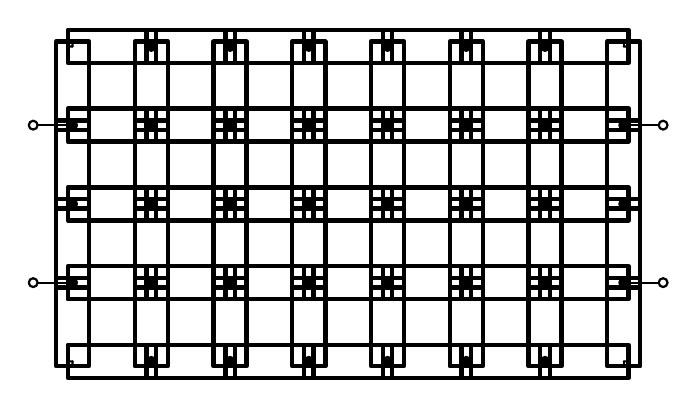
\begin{tikzpicture}
      \def\ROW{1,2,3,4,5}
    \def\COL{1,2,3,4,5,6,7}
    \foreach \j in \ROW {
      \foreach \i in \COL {
          \draw (\i,\j) to [R] (\i+1,\j);
      }
      }  
      \def\ROW{2,3,4,5}
    \def\COL{1,2,3,4,5,6,7,8}  
    \foreach \j in \ROW {
      \foreach \i in \COL {
      \draw (\i,\j) to [R] (\i,\j-1);
      }
      }
    % dots
      \draw (0.5,4) to[short,o-*] (1,4);  
    \draw (0.5,2) to[short,o-*] (1,2);
    \draw (8,4) to[short,*-o] (8.5,4);  
    \draw (8,2) to[short,*-o] (8.5,2);
    
    \draw (8,3) to[short,*-] (8,3);
    \draw (1,3) to[short,*-] (1,3);
  
      \def\ROW{1,2,3,4,5}
    \def\COL{2,3,4,5,6,7}  
      \foreach \j in \ROW {
      \foreach \i in \COL {
      \draw (\i,\j) to [short,*-] (\i,\j);
      }
      }  
  \end{tikzpicture}
%  \caption{Pasivní dvojbran v podobě husté vodivostní sítě}\label{ES:fig_res_grid}
%\end{figure}
\end{document} 